\section{Decomposição de vizinhanças (Disaggregated Neighborhoods)} \label{subsec:metodologiaDecomposicaoVizinhancas}

Pela Figura~\ref{fig:dvndGraph} podemos perceber que o paralelismo horizontal, isto é, aquele obtido pela utilização de mais máquinas, neste método está limitado a quantidade de vizinhanças utilizadas no método DVND.
Esta limitação representa um problema pois para obter melhor utilização do paralelismo horizontal seria necessário também adicionar novas estruturas de vizinhanças, o que aumentaria o esforço computacional e não necessariamente traria ganho de performance ou na qualidade do valor da solução.

Contudo este problema pode ser facilmente solucionado pela decomposição das vizinhanças, isto é, no lugar de um nó \textit{oper} representar toda uma estrutura de vizinhança, este passa a processar uma sub-parte desta.
% Por exemplo, na Figura~\ref{fig:operadorSwap} temos uma vizinhança de tamanho $\mathcal{O}(n^2)$ em que cada elemento é trocado com todos os elementos subsequentes, conforme pode ser visto na Figura~\ref{fig:vizinhancaTrocas} cada elemento tem um grupo independente de trocas.

\begin{figure}[htbp]
    \centerline{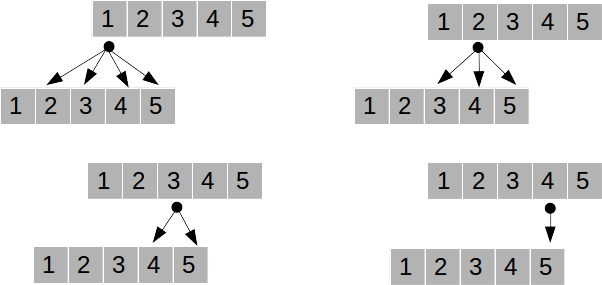
\includegraphics[scale=0.6]{figuras/vizinhanca.png}}
    \caption{Vizinhança com suas trocas para $n=5$.}
    \label{fig:vizinhancaTrocas}
\end{figure}

Isto posto, podemos separar a vizinhança em sub-grupos, um exemplo poderia ser a Figura~\ref{fig:vizinhancaTrocasDividida} que mostra a mesma vizinhança da Figura~\ref{fig:vizinhancaTrocas} dividida em dois sub-grupos. Desta forma cada sub-grupo representaria um nó \textit{oper} do diagrama dataflow DVND aumentando assim a escalabilidade horizontal do método.

\begin{figure}[htbp]
    \centerline{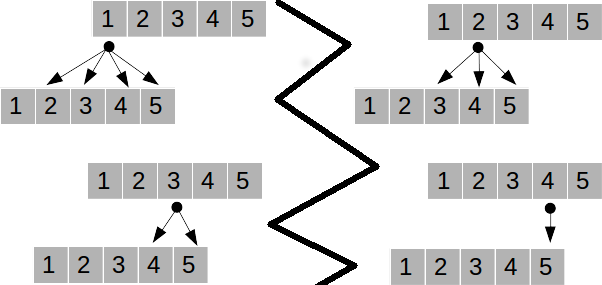
\includegraphics[scale=0.6]{figuras/vizinhancaDividida.png}}
    \caption{Vizinhança com suas trocas dividida para $n=5$.}
    \label{fig:vizinhancaTrocasDividida}
\end{figure}

A vizinhança na Figura~\ref{fig:vizinhancaTrocasDividida} exemplifica a sub-divisão em dois grupos de vizinhança contudo esta divisão limita-se apenas ao tamanho da solução proporcionando um grande potencial para o desenvolvimento do paralelismo horizontal de qualquer vizinhança sem aumentar demasiadamente o custo computacional do método.
